%!TEX root = project.tex

\chapter{Methodology}

\begin{itemize}
%\item Agile / incremental and iterative approach to development. Planning, meetings.
\item What about validation and testing? Junit or some other framework.
\item If team based, did you use GitHub during the development process.
\item Selection criteria for algorithms, languages, platforms and technologies.
\end{itemize}

\begin{figure}[H]
    \centering
    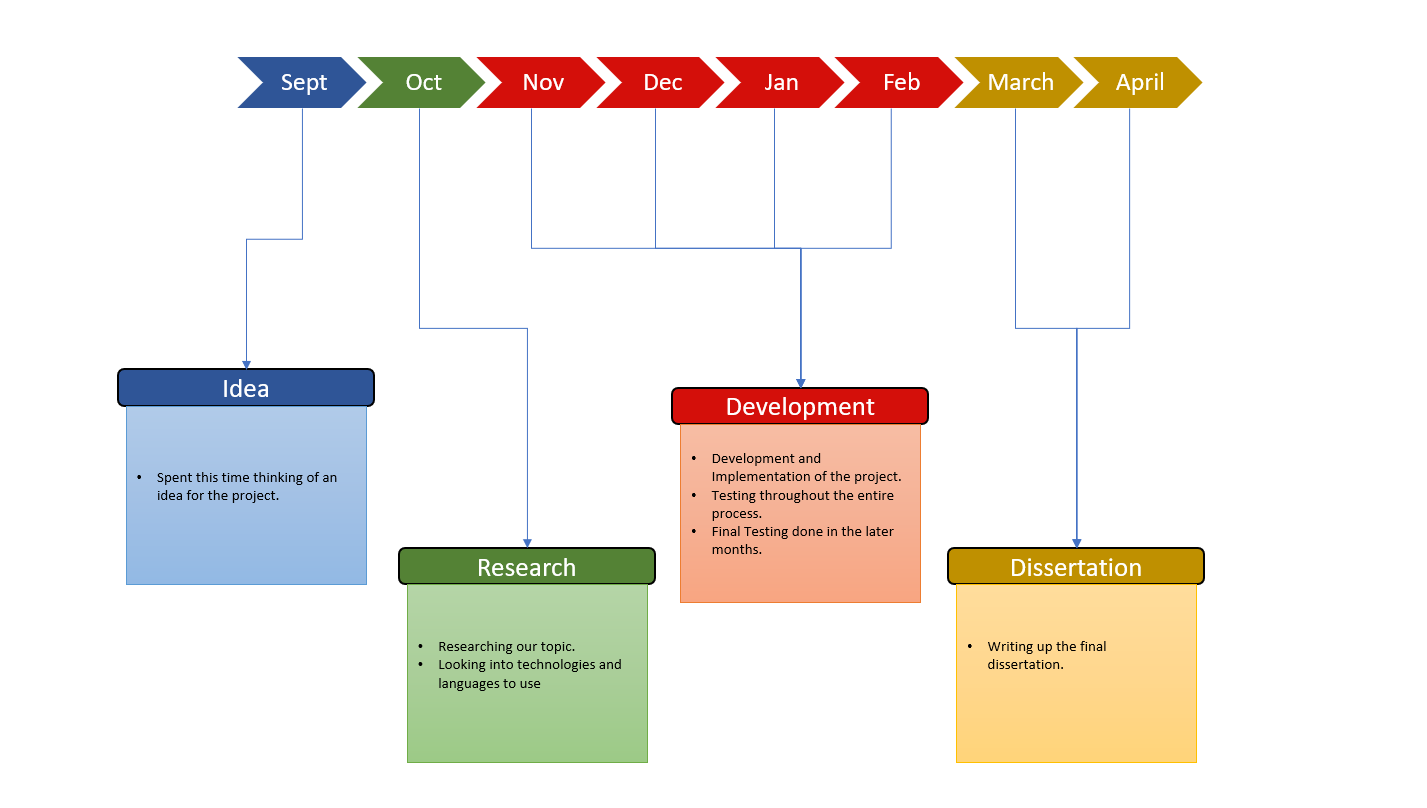
\includegraphics[width=140mm, height=70mm]{img/timeline.PNG}
    \caption{Project Timeline}
    \label{fig:timeline}
\end{figure}

\section{Overview}
In this section we will review our approach to the project development, describe the methodology used and how it was implemented and how the development of the project progressed overall. At the conclusion of this methodology the reader should be left with a good sense of the project scale, as well as the steps taken throughout.

For this project we wanted to use an iterative design process, so changes and issues could easily be kept track of and dealt with in an easy and efficient manner. As such we felt the Agile method to be the best fit for us, as one of the team members has had previous experience in industry during a summer internship. His first hand experience helped guide us throughout the project, and gave the rest of us a feel on how it may be like to work in industry in the future.

The Agile method is a particular approach to project management, which is ubiquitous in the environment of Software Development. This method assists teams in responding to the unpredictability of constructing software, such as bugs in code, changing requirements from the client, etc. Agile uses incremental/iterative work sequences commonly known as Sprints, which is a period of time allocated for a particular phase of a project. Time is a precious resource when developing software, and as such a Sprint is considered complete once the time period expires. While some objectives set out for the Sprint may not have been realised, these additions will need to be put on the back burner in order to keep up with the Agile development cycle.

While we liked the approach the Agile method allowed us to use, we did not adhere to it in the strictest of senses. For instance, we did not appoint someone to the role of Scrum Master, preferring a more group oriented approach to problem solving and troubleshooting. A Scrum Master would be more suited to an industry environment, where they could be used as a point of contact or cohesion between large teams with differing responsibilities.

Another aspect of the Agile Methodology we utilized were "Stand ups". This is the term used for a daily progress meeting, traditionally held within a development area. These meetings are a quick way to gauge progress on individual aspects of a project, and are a great way to keep everyone informed and motivated. (once or twice a week for stand ups, library room, discuss work individually. Well informed anyways)

Some general principles of Agile include:

\begin{itemize}
    \item{Satisfy the client and continually develop software}
    \item{Changes in requirements are embraced}
    \item{Frequent delivery of working software} 
    \item{Close working relationship between client and developer(s)}
    \item{Face to face communication is integral to cohesive development, and working relations as a whole}
\end{itemize}

\section{Sprint 1: Idea}
	
	Our first sprint was used to spitball potential ideas for a project, including what problem could we tackle, relevant technologies we could apply to said problem and in what manner we could approach it.
	
	A particular point we needed to take note of was the scope of the project. The project would need to encompass a number of technologies that were not only relevant in relation to our course or module, but also technologies that are being used in day to day applications. 
	
	As noted in our "Ideas" subsection, we stumbled across a video from an event called the "Robocup", in which Artificially Intelligent robots competed in a game of football. Finding this video was the seminal point in our project, where we collectively agreed that agents controlled by Artificial Intelligence was a valid route to go down. With our idea firmly in place it was time to move onto the research phase, in which we searched for relevant platforms, technologies and languages.
	
\section{Sprint 2: Research}
	
	The next Sprint focused on researching our materials for the project, such as a suitable environment we could use, what languages we could utilize and if there were any external libraries or resources we could use to improve the overall scope.
	
	The types of research undertaken in this sprint ranged from articles, videos, Stack Overflow forum posts and peer-to-peer, asking colleagues about their previous experiences with certain technologies. We also reviewed many technologically related papers through the use of Google Scholar and the GMIT Library site.
	
	For our environment we settled on the Unity game engine, in which we had some previous experience in a different module. This environment allowed us to create a 3D framework for the agents, so progress could be visualized as well as documented in a traditional way. For our language of choice we settled on Python, due to the apparent ubiquity of the language in machine learning and data modelling circles, as well as the comprehensive standard library and open source libraries it offered.

	The ML-Agent Toolkit is an open-source Unity plugin that enables games and simulations to serve as environments for training intelligent agents. We felt the addition of the Toolkit would take much of the hassle out of creating a machine learning framework ourselves.To still make use of the Python language itself we made used  Jupyter Notebooks to pass information to and from unity/ML-Agents. We also had previous experience with Jupyter Notebooks from another module, so felt comfortable working with this program.
	More information on this subject can be found later, in the "Technology" section.With the basics gathered it was time to move onto initial development.
	

\section{Sprint 3: Initial Development}
	Set up environment, GitHub, etc
	
	Once we had established a framework we were happy with work finally began on the foundations of the project. To tackle the problem of version control we utilized GitHub, which we have had extensive experience using in the past. Group members were then added as collaborators, so we could work on the project in unison.  Once the blank Unity environment was created it was pushed to the GitHub, as well as any relevant research materials we had to date.
	
	The task of setting up the Jupyter Notebooks, Unity and ML-Agents fell to Ryan, Brian and James respectively.
	
	Documentation on ML-Agents was scoured over in order to integrate it into Unity, which required the use of the Jupyter Notebooks themselves. It was at this stage the team understood how interconnected these individual processes needed to be in order for the project to operate efficiently.
	
	An environment in Unity was created for our initial testing purposes, namely a small football pitch with translucent walls and a ceiling, so any chances of assets "escaping" the testing area were minimized. This environment also contained the two goals that would be used by the opposing teams. Next came the creation of other assets, namely the ball itself and the first agents. By now the project seemed to be taking shape. Next, we move onto integration and testing.
	
	

\section{Sprint 4: Integration and Testing}
	Integration testing of ML-Agents, Unity, Notebooks, etc
	
	The next sprint focused on the integration and testing of the various technologies and platforms we had chosen. 
	
	The application works by using Unity to "host" the ML-Agents toolkit, as it is essentially a Unity add-on in itself. Data within the ML-Agents Toolkit is passed to and from the Jupyter notebooks. The Notebook is used as a connector, staging blocks of code to execute in sequence so Unity doesn't become overloaded, as well as ease of debugging later.
	
	After some time testing and debugging we finally had all three individual components integrated into one cohesive application. During this time we passed random values to the agents in the environment, in order to test the robustness of the Jupyter Notebooks in passing values, and to see how the agents reacted in the environment.
	
	One issue encountered during this sprint was in relation to ML-Agents, and how GitHub handles large files. This caused a blocking issue within the sprint, which meant all of the members of our team could not progress until this issue was resolved. 
	
	This issue was eventually resolved by adding the necessary folder to a public google drive address that anyone can access. The wiki on the GitHub page explains how to implement this folder into the project and contains a link to the google drive where it is stored.


\section{Sprint 5: Functionality and Testing}
	
	This Sprint focused on the crux of the project, controlling agents in a meaningful manner using Artificial Intelligence, and also where we encountered our issue. These issues can be read about in detail below, in the "Conclusion" section. 
	
	During this time we focused on a final code review, adding elements that we felt were necessary in order to explain our project and its intentions, or adding more to our current code base and design in order to provide clarity.
	Time was also spent making note of areas in which our project or write up may not have been up to scratch, and added any issues to the workload for the final sprint.


\section{Sprint 6: Cleanup \& Dissertation} 

	The final Sprint was focused on project cleanup, as well as work on our accompanying minor dissertation. This time was spent implementing our research into the dissertation, as well as relevant images, graphs, blurbs and context to our approach.  
